\item[(f)]
\section{Tolerance Scheme and Filter Order}

\subsection*{Problem Statement}
Is the tolerance scheme being violated? Can the tolerance scheme be fulfilled by increasing the filter order to \( N = 90 \)?

\subsection*{Theoretical Background}
The tolerance scheme specifies the allowable deviations in the passband and stopband of the filter's frequency response. By comparing the frequency response of the designed FIR filter with the specified tolerance scheme, we can determine if the scheme is violated. Increasing the filter order typically results in a sharper transition band and improved adherence to the tolerance scheme.

\subsection*{Analysis}

\subsubsection*{Current Filter Order \( N = 20 \)}
The frequency response of the FIR filter with \( N = 20 \) was previously plotted. By examining this plot, we can check for any violations of the tolerance scheme in the passband ripple and stopband attenuation.

\subsubsection*{Increased Filter Order \( N = 90 \)}
An FIR filter with \( N = 90 \) is designed using the same method (rectangular window). The frequency response is computed and plotted to determine if it meets the tolerance scheme requirements.

\subsection*{Implementation and Results}
The frequency response of the FIR filter with \( N = 90 \) is computed and plotted using Python. The plot below illustrates the frequency response along with the specified tolerance scheme.

\begin{figure}[h]
    \centering
    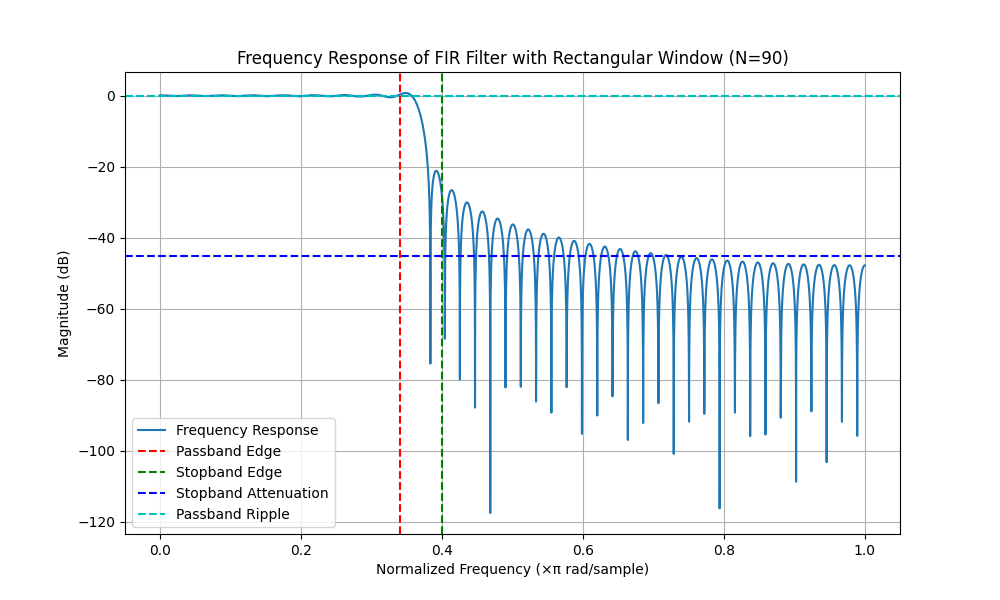
\includegraphics[width=0.8\textwidth]{fig/ex4_f_frequency_response_90.png}
    \caption{Frequency Response of FIR Filter with Rectangular Window (N=90)}
    \label{fig:ex4_f_frequency_response_90}
\end{figure}

\subsection*{Conclusion}
By comparing the frequency response plots for \( N = 20 \) and \( N = 90 \), we can determine if the tolerance scheme is violated for \( N = 20 \) and if increasing the filter order to \( N = 90 \) fulfills the tolerance scheme requirements.
